\documentclass[11pt,spanish]{article}

\usepackage{listings}             
\usepackage{anysize} 
\usepackage{graphicx}
\usepackage[spanish,mexico]{babel}
\usepackage[utf8]{inputenc}
\usepackage{xcolor}
\usepackage{wrapfig}



\lstset{language=Python}
\marginsize{1cm}{1cm}{2cm}{2cm}
\selectlanguage{spanish}
\lstset{
language=Python,
 backgroundcolor=\color{red!75!green!50!blue!25},
 frame=single,
literate=
  {á}{{\'a}}1 {é}{{\'e}}1 {í}{{\'i}}1 {ó}{{\'o}}1 {ú}{{\'u}}1
  {Á}{{\'A}}1 {É}{{\'E}}1 {Í}{{\'I}}1 {Ó}{{\'O}}1 {Ú}{{\'U}}1
  {à}{{\`a}}1 {è}{{\`e}}1 {ì}{{\`i}}1 {ò}{{\`o}}1 {ù}{{\`u}}1
  {À}{{\`A}}1 {È}{{\'E}}1 {Ì}{{\`I}}1 {Ò}{{\`O}}1 {Ù}{{\`U}}1
  {ä}{{\"a}}1 {ë}{{\"e}}1 {ï}{{\"i}}1 {ö}{{\"o}}1 {ü}{{\"u}}1
  {Ä}{{\"A}}1 {Ë}{{\"E}}1 {Ï}{{\"I}}1 {Ö}{{\"O}}1 {Ü}{{\"U}}1
  {â}{{\^a}}1 {ê}{{\^e}}1 {î}{{\^i}}1 {ô}{{\^o}}1 {û}{{\^u}}1
  {Â}{{\^A}}1 {Ê}{{\^E}}1 {Î}{{\^I}}1 {Ô}{{\^O}}1 {Û}{{\^U}}1
  {œ}{{\oe}}1 {Œ}{{\OE}}1 {æ}{{\ae}}1 {Æ}{{\AE}}1 {ß}{{\ss}}1
  {ű}{{\H{u}}}1 {Ű}{{\H{U}}}1 {ő}{{\H{o}}}1 {Ő}{{\H{O}}}1
  {ç}{{\c c}}1 {Ç}{{\c C}}1 {ø}{{\o}}1 {å}{{\r a}}1 {Å}{{\r A}}1
  {€}{{\EUR}}1 {£}{{\pounds}}1
}



\title{\vspace{-3cm}\begin{flushleft}\textbf{Actividad 1}\end{flushleft}}
\author{\hspace{-9.6cm}\textsc{Andrés Ignacio Rodríguez Mendoza}}
\date{}

\begin{document}

\begin{wrapfigure}{r}{0.2\textwidth}
  \begin{center}
   \vspace{-5.2cm} 
\includegraphics[width=0.15\textwidth]{uni}
  \end{center}
\end{wrapfigure}

\maketitle  
\begin{center}
\rule{\textwidth}{1pt}
\end{center}

Las matemáticas de péndulos son, en general, bastante complicadas. Se realizan supuestos para simplificar el modelo, que en el caso del péndulo simple permite a las ecuaciones de movimientos ser resueltas analíticamente para oscilaciones pequeñas.
	






\section*{Péndulo simple}
El llamado  ``péndulo simple'' es una idealización de un ``péndulo real'' en un sistema aislado usando los siguientes supuestos:
\begin{itemize}
	\item Se considera una cuerda sin masa, inextensible y siempre tensa.
	\item El objeto es una masa puntual.
	\item El movimiento ocurre en dos dimensiones.
	\item Se desprecia fricción o resistencia al aire.
	\item el campo gravitacional es uniforme.
	\item El soporte está fijo.
\end{itemize}
La ecuación diferencial que representa el movimiento de un péndulo simple es

\begin{equation}
\frac{d^2\theta}{dt^2} + \frac{g}{l} \sin \theta = 0
\end{equation}\\
donde g es la aceleración debido a la gravedad, $l$ es la longitud de la cuerda, y $\theta$ es el desplazamiento angular.\\

\begin{figure}[h]
\centering
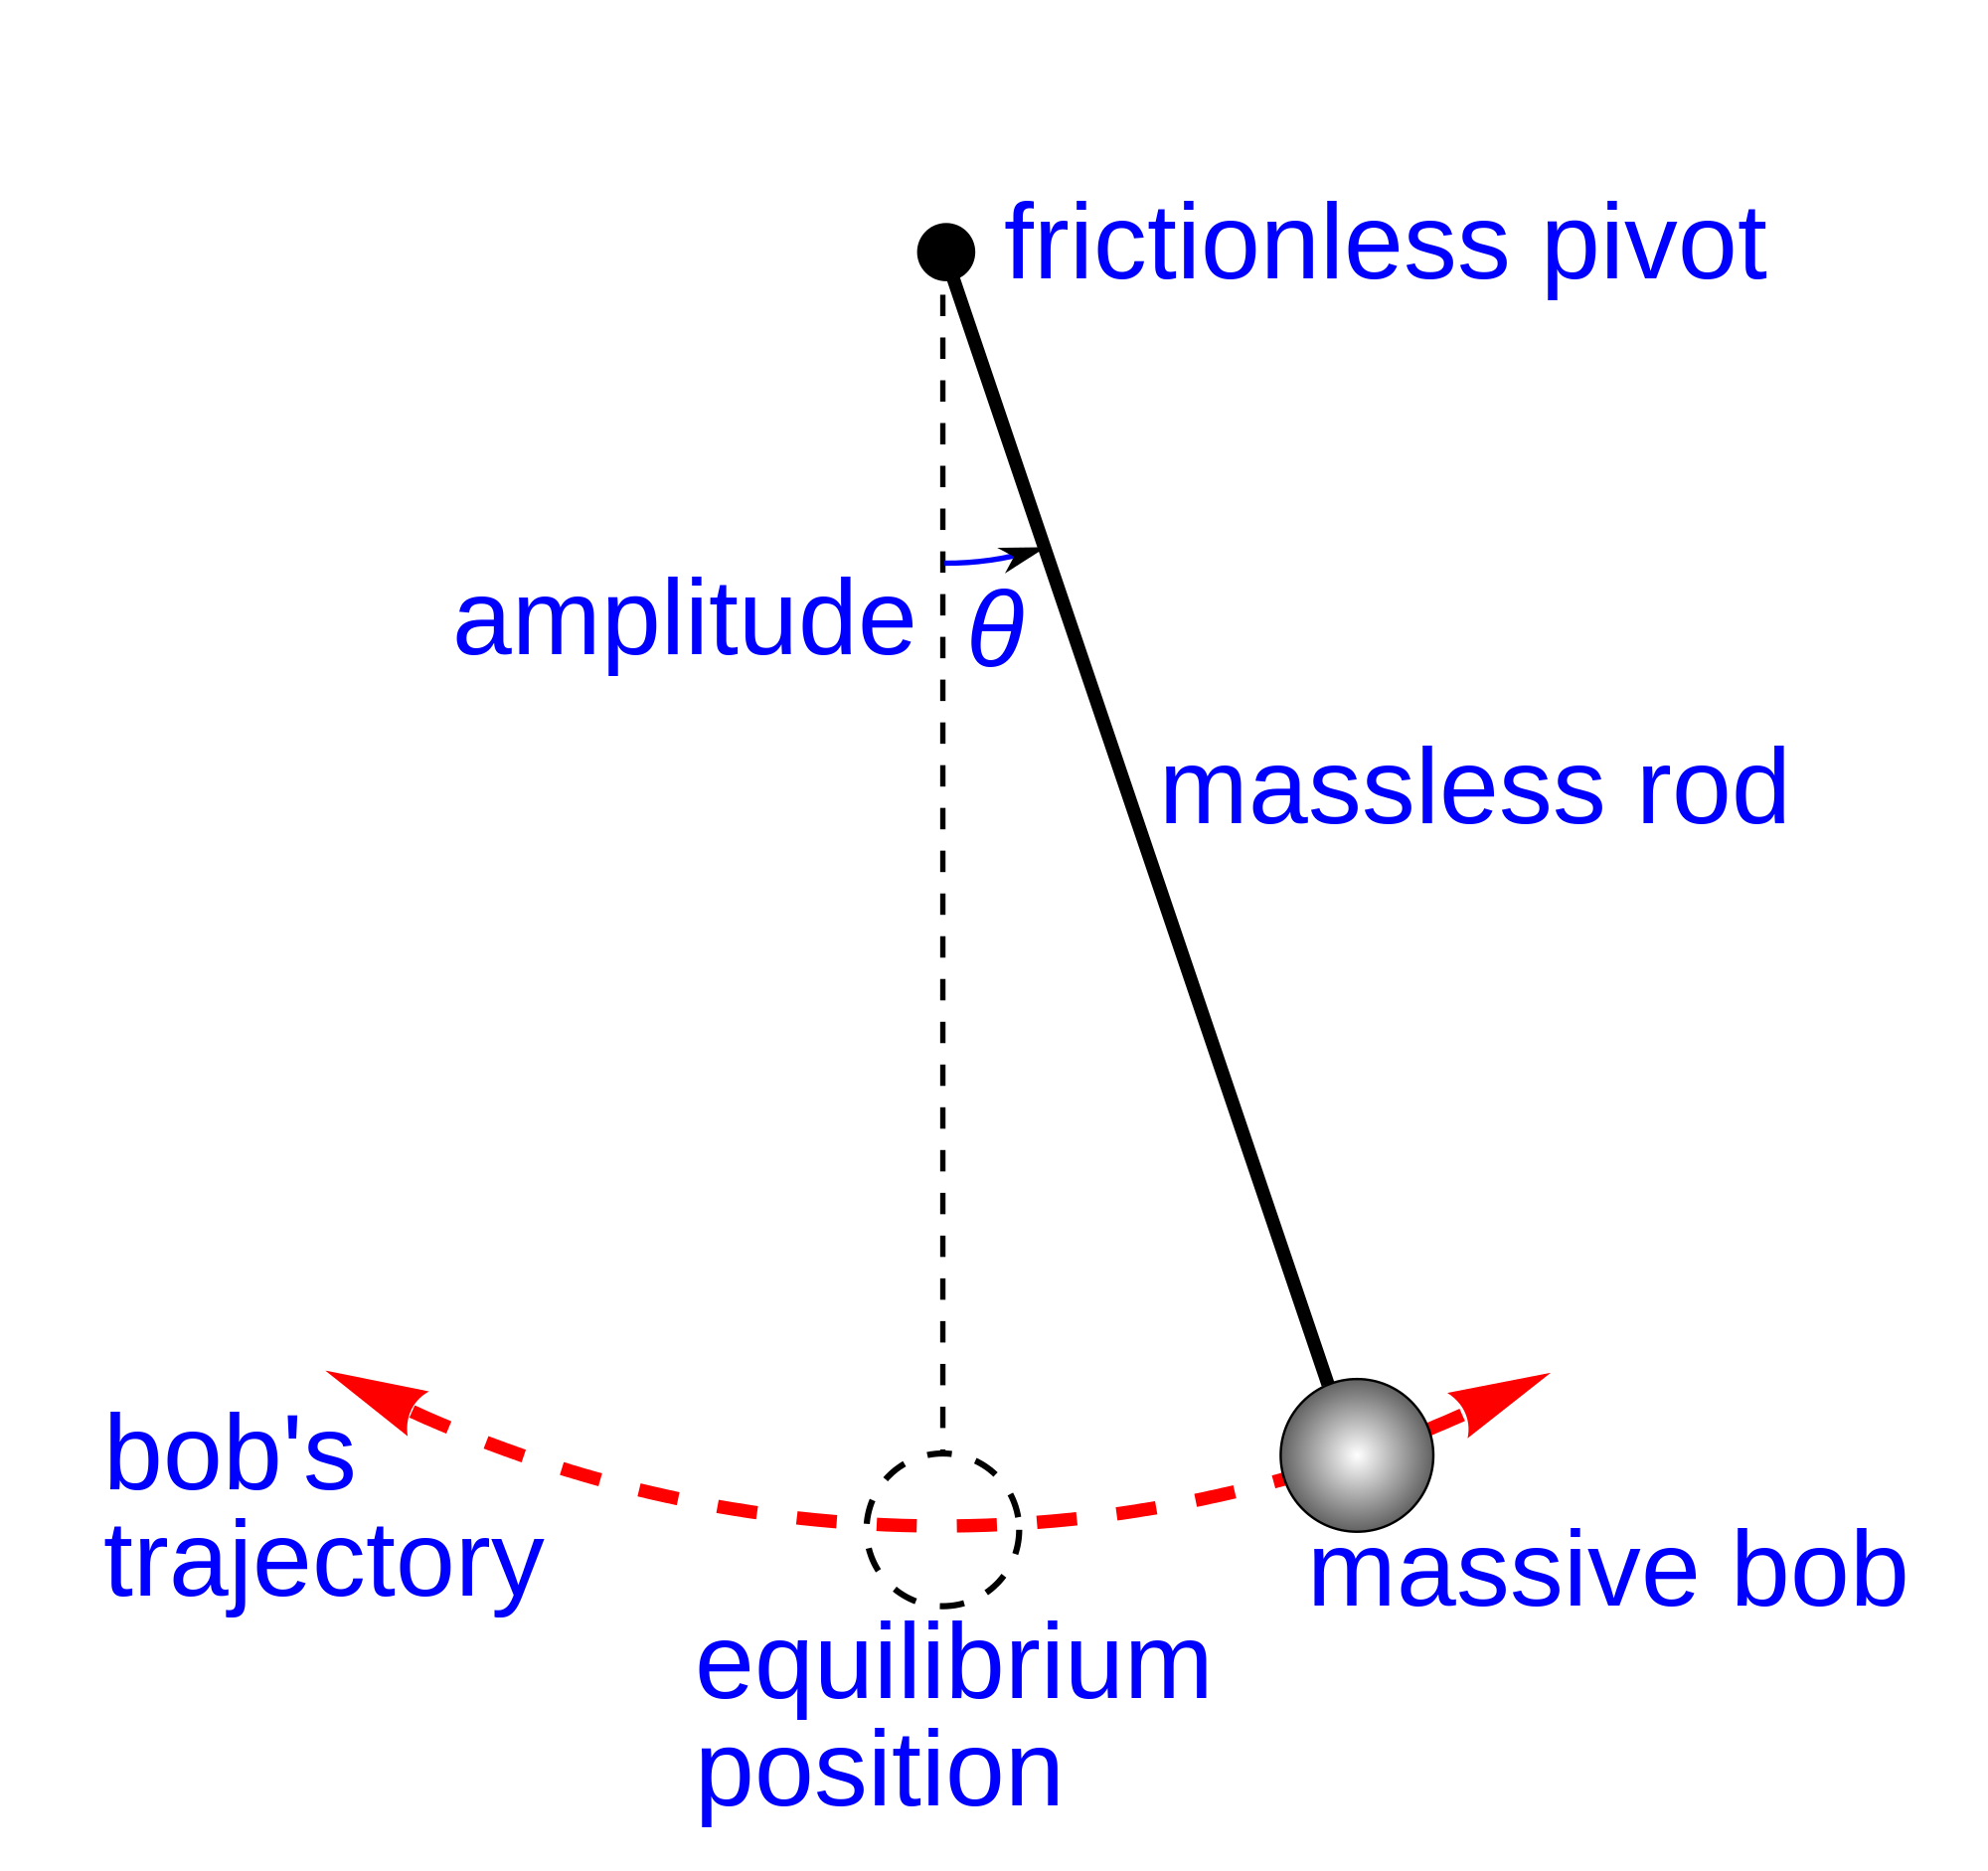
\includegraphics[scale=0.1]{pend}
\caption{Péndulo simple}
\end{figure}

\section*{Aproximación para ángulos pequeños}

La ecuación diferencial no es resuelta tan facilmente como considerando ángulos más pequeños que un radián, es decir, $\theta \ll  1$, por lo cual, $\sin \theta \approx \theta$. Reemplazando esto en la ecuación diferencial, queda,

\begin{equation}
\frac{d^2\theta}{dt^2} + \frac{g}{l} \theta = 0.
\end{equation}\\
Dadas las condiciones iniciales $\theta (0) = \theta _ 0$ y $d\theta / dt (0) =0$, la solución es,
\begin{equation}
\theta (t) = \theta _0 \cos \left( \sqrt{\frac{g}{l} t} \right)
\end{equation}\\
El movimiento es un movimiento armónico simple, donde $\theta_0$ es la semiamplitud de oscilación. El periodo del movimiento es,

\begin{equation}
	T_0 = 2 \pi \sqrt{\frac{l}{g}}.
\end{equation}

\section*{Periodo de amplitud arbitraria}

Para amplitudes más grandes que la aproximación a ángulos pequeños, se puede calcular el periodo invirtiendo la ecuación de la velocidad angular,

\begin{equation}
\frac{dt}{d\theta}=\frac{l}{2g} \frac{1}{\sqrt{\cos \theta - \cos \theta_0}}
\end{equation}\\
e integrando sobre un ciclo completo,
$$ T= t(\theta _0 \rightarrow 0 \rightarrow -\theta_0 \rightarrow 0 \rightarrow \theta_0),$$\\
o dos veces un medio ciclo,
$$ T= 2t(\theta _0 \rightarrow 0 \rightarrow -\theta_0),$$\\
o cuatro veces un cuarto de ciclo,
$$ T= 2t(\theta _0 \rightarrow 0),$$\\
que nos lleva a
\begin{equation}
T= 4 \sqrt{\frac{l}{2g}} \int ^{\theta _0} _0 \frac{1}{\sqrt{\cos\theta - \cos\theta_0}} d\theta.
\end{equation}\\
Nótese que esta integral diverge como $\theta_0$ se aproxime a la vertical. Así, con la energía adecuada, un péndulo en su máximo podría tomar un tiempo arbitrariamente largo para caer.

\end{document}


\maketitle